\documentclass[9pt]{IEEEtran}

\usepackage[english]{babel}
\usepackage{graphicx}
\usepackage{epstopdf}
\usepackage{fancyhdr}
\usepackage{amsmath}
\usepackage{amsthm}
\usepackage{amssymb}
\usepackage{url}
\usepackage{array}
\usepackage{textcomp}
\usepackage{listings}
\usepackage{hyperref}
\usepackage{xcolor}
\usepackage{colortbl}
\usepackage{float}
\usepackage{gensymb}
\usepackage{longtable}
\usepackage{supertabular}
\usepackage{multicol}

\usepackage[utf8x]{inputenc}

\usepackage[T1]{fontenc}
\usepackage{lmodern}
\input{glyphtounicode}
\pdfgentounicode=1

\graphicspath{{./figures/}}
\DeclareGraphicsExtensions{.pdf,.png,.jpg,.eps}

% correct bad hyphenation here
\hyphenation{op-tical net-works semi-conduc-tor trig-gs}

% ============================================================================================

\title{\vspace{0ex}
Model evaluation}

\author{Marko Medved\vspace{-4.0ex}}

% ============================================================================================

\begin{document}

\maketitle

\section{Cross-Validation}
Cross-validation was implemented and evaluated on four different models. 
The performance of each model was assessed using log loss and accuracy as
 evaluation metrics.
\subsection{Implementation details}
Since the dataset is assumed to be representative of the data generating process 
and the target class distribution
is imbalanced, stratified cross-validation was implemented. This ensures that eac
 fold maintains the same class distribution as the overall dataset, preventing the
  learning algorithm from encountering folds where certain classes are 
  underrepresented. Preserving class balance ensures the model can learn 
  patterns from all classes, leading to more reliable evaluation.
\\
As instructed, a baseline classifier and logistic regression were first
 evaluated. For the third model, a decision tree was chosen due to its 
 sensitivity to the minimum number of observations required to split a node —
  a key parameter that was optimized within each fold.

The parameter optimization was carried out in two ways:

\begin{itemize}
    \item \textbf{Training Fold Optimization:} Trained on the training split of each fold; the parameter that produced the lowest log loss was selected.
    \item \textbf{Nested Cross-Validation:} Applied an additional layer of cross-validation within the training split. The parameter with the lowest cumulative log loss from the inner folds was selected.
\end{itemize}

Log loss was chosen as the evaluation metric instead of accuracy because it
 is a strictly proper scoring rule — meaning it encourages the model to output
  the true class probability distribution as opposed to accuracy where only the mode of the distribution 
  is taken into account.
\\
The choice of k = 10 for cross-validation was made because decision trees are 
inherently unstable models — they are sensitive to small variations in the 
training data, which can increase variance when using a larger k. Since the
 dataset is reasonably large, 10 folds strike a good balance between bias and
  variance, providing a stable estimate of model performance without
   introducing excessive bias from smaller training sets.

A similar reasoning applies to the inner loop of the nested cross-validation. 
With only 10\% less data available in the inner loop compared to 
the outer loop, using the same value of k (10) should still maintain 
 an effective balance between training size and validation 
stability.

\subsection{Results}
Table~\ref{tab:results} shows the performance of the four models. 
Note that the uncertainty was quantified using bootstrap with 500 repetitions.

Focusing on log loss, the decision tree shows a particularly high value,
 especially when using training fold optimization. This can be attributed
  to the fact that this model is often overly confident in its predictions, 
  meaning the predicted class tends to have a very high probability.
   Consequently, in the case of misclassification, this high confidence
    leads to a larger penalty, resulting in high log loss.
     This effect is especially evident when using training fold 
     optimization, where the tree overfits more severely than in the
      nested CV case. Note that the smallest possible minimal number
       of observations required to split a node during parameter tuning
        was set to 10, which helps prevent the tree from completely 
        overfitting.

When examining accuracy, the results are more consistent when 
compared to logistic regression, which is expected since accuracy only
 considers the predicted class and not the full predicted distribution.



 \begin{table}[h]
    \begin{tabular}{l|l|l}
    Model                           & Log loss& Accuracy          \\
    \hline
    Baseline       & 1.161 $\pm$ 0.013    & 0.6121 $\pm$  0.0069          \\
    Logistic Regression       & 0.672 $\pm$ 0.013 & 0.7329 $\pm$   0.0060               \\
    Decision Tree  &  2.569 $\pm$ 0.095  & 0.7217 $\pm$ 0.0063                \\
    Decision Tree (Nested CV)  &1.378 $\pm$ 0.059 & 0.7386 $\pm$ 0.0060  
    \end{tabular}
    \vspace{2px}
    \caption{Performance Comparison of Models}
    \label{tab:results}
\end{table}

\section{Effect of Distance on Error}
To investigate the influence of distance on errors, two different methods 
were applied.
\\
Firstly, a visual method involved plotting a scatter plot of log losses at 
different distances, along with a fitted linear regression trend shown in
 Figure~\ref{fig:error_distance}. The plot includes results for all models,
  where we observe a general trend of decreasing log loss at larger distances.
For the baseline model, the plot may appear unusual; however, this is 
expected since the number of distinct log losses is limited by the number
 of shot types.

 \begin{figure}[h]
    \centering
    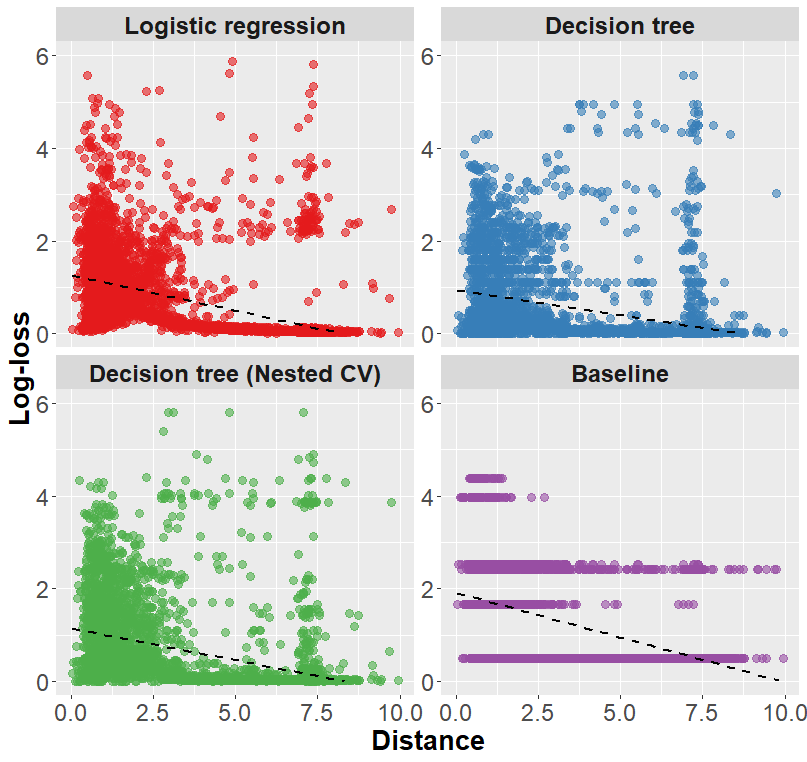
\includegraphics[width=0.95\columnwidth]{figures/distance_error.png}
    \caption{Effect of Distance on Log-Loss Across Models}
    \label{fig:error_distance}
\end{figure}

 The second method involved calculating the correlation coefficient between 
 distance and log loss to quantify their linear relationship. As shown in 
 Table~\ref{tab:correlation}, all four models produced a negative correlation
  coefficient, indicating that log loss tends to decrease with increasing 
  distance, consistent with the visual observation.


\begin{table}[h]
    \begin{tabular}{l|l}
    Model                           & Correlation          \\
    \hline
    Baseline       & -0.562 $\pm$  0.009            \\
    Logistic Regression       & -0.455 $\pm$ 0.018              \\
    Decision Tree  &  -0.311 $\pm$  0.009            \\
    Decision Tree (Nested CV)  &-0.245 $\pm$  0.008
    \end{tabular}
    \vspace{2px}
    \caption{Correlation Between Distance and Log-Loss Across Models}
    \label{tab:correlation}
\end{table}
This relationship can be explained by examining the distribution of shot types. 
Figure~\ref{fig:shot_distr} shows that at higher distances, most shots are classified
 as above head shots, whereas the distribution is more balanced in the overall dataset
  and at lower distances. For high-distance shots, the top 25\% of distances were selected, 
  while for low-distance shots, the bottom 25\% were used. This also explains why 
  the baseline model exhibits the highest correlation, since it always assignes the highest 
  probability to the majority class.

\begin{figure}[h]
    \centering
    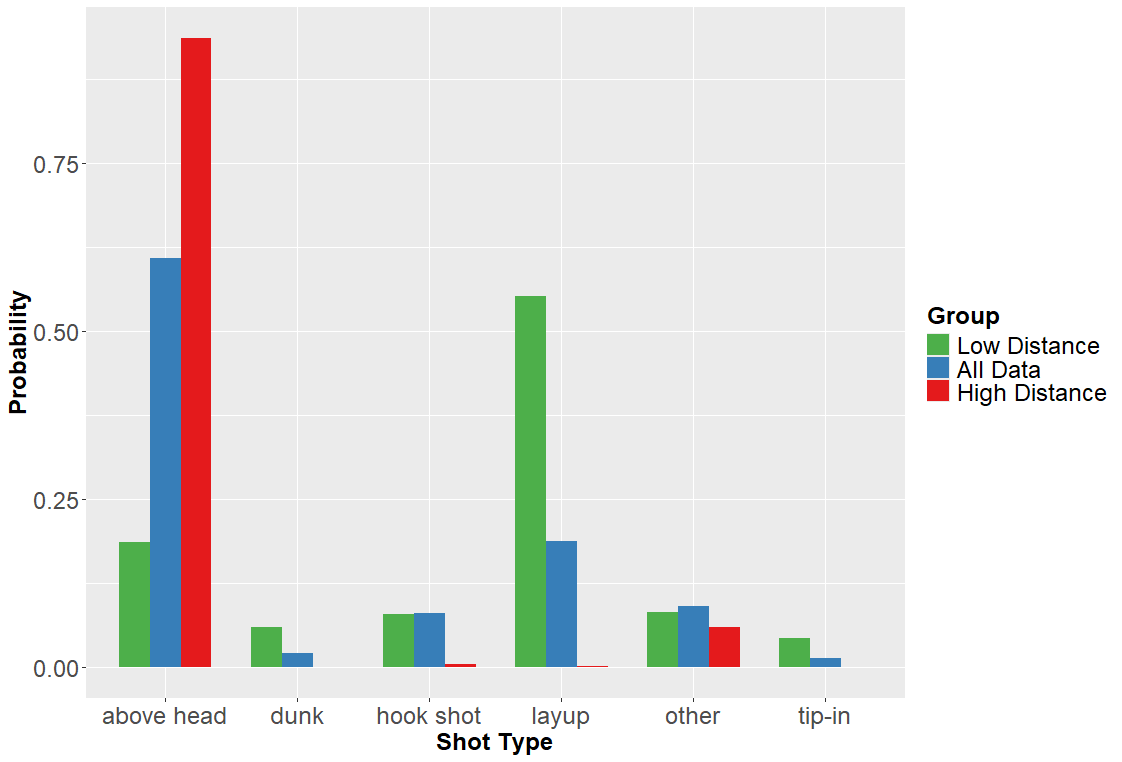
\includegraphics[width=0.95\columnwidth]{figures/shot_distr.png}
    \caption{Shot Type Distribution By Distance}
    \label{fig:shot_distr}
\end{figure}


\section{Estimating performance on True Competition Distribution}
\subsection{Implementation details}

To estimate how our model would perform on the true distribution of
 competition types, a weighted bootstrap method was implemented.

Unlike standard bootstrap, where samples are drawn uniformly, the 
weighted bootstrap adjusts the sampling probabilities based on the 
difference between the true and observed class distributions.
Specifically, the sampling weights were calculated by taking the 
ratio of the true class probability (for competition types) to the 
current class probability. The weights were then normalized by dividing 
by their sum to create a valid probability distribution.

This approach ensures that the bootstrap samples reflect the true 
distribution of competition types, providing a more accurate estimate 
of model performance. Note that this method was applied directly to the 
log-losses and accuracies calculated in the first part.

\subsection{Results}
Table~\ref{tab:results_true} shows the results of this 
estimation. The results differ slightly from the original ones, with 
most models showing a slight improvement — particularly the baseline 
model, which demonstrates noticeably better performance.

\begin{table}[h]
    \begin{tabular}{l|l|l}
    Model                           & Log loss& Accuracy          \\
    \hline
    Baseline       & 1.126 $\pm$ 0.013    &  0.6351 $\pm$  0.0068          \\
    Logistic Regression       &  0.652 $\pm$ 0.013 & 0.7525 $\pm$ 0.0061               \\
    Decision Tree  &  2.599 $\pm$ 0.094  & 0.7298 $\pm$ 0.0063                \\
    Decision Tree (Nested CV)  & 1.368 $\pm$ 0.060 &  0.7490 $\pm$ 0.0062  
    \end{tabular}
    \vspace{2px}
    \caption{Performance Comparison on True Competition Distribution}
    \label{tab:results_true}
\end{table}

To explain this, we need to revisit the distribution of shot types — this time in 
relation to the competition type, as shown in Figure~\ref{fig:shot_distr_comp}. By 
adjusting the data to reflect the true distribution, we increased the influence of data
 points from the NBA competition type while reducing the influence of others.

Since the above head shot type is more frequent in NBA data points, it is not 
suprising that the performance of the baseline model improved.

 \begin{figure}[h]
    \centering
    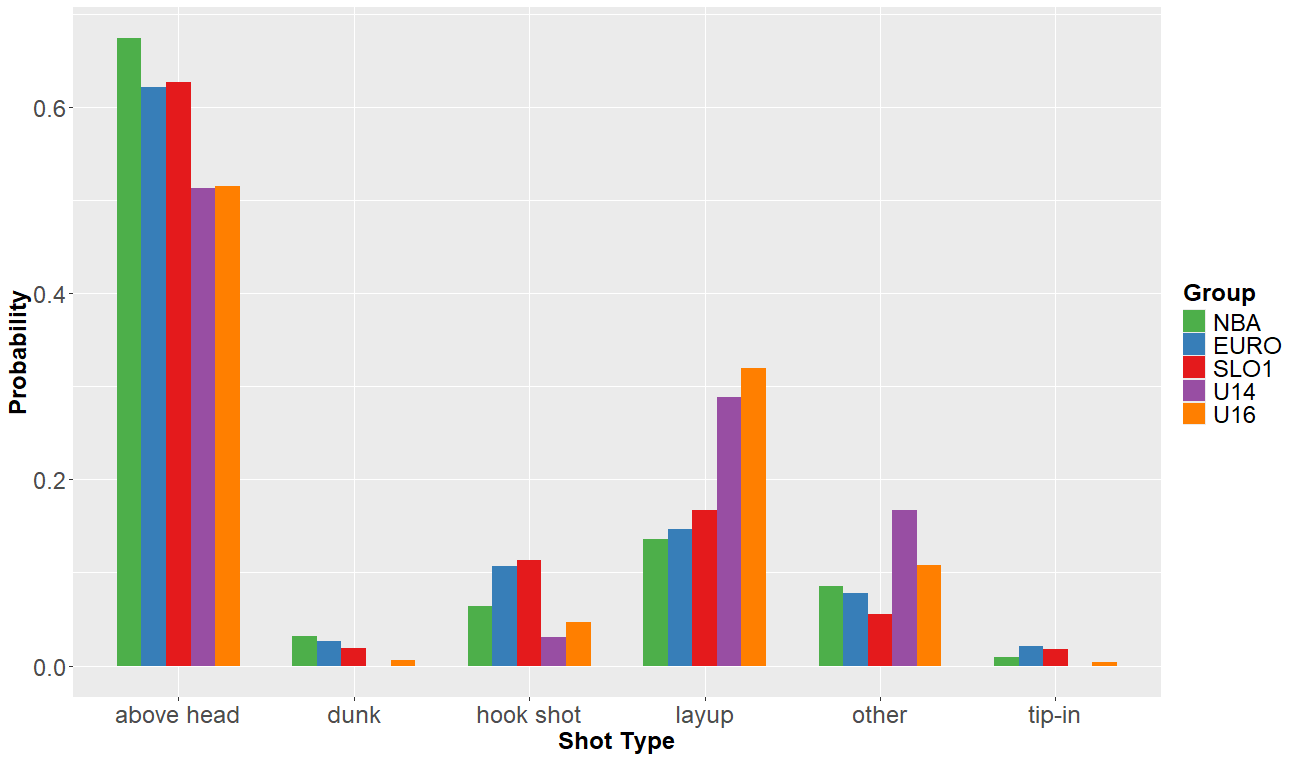
\includegraphics[width=0.95\columnwidth]{figures/shot_distr_comp.png}
    \caption{Shot Type Distribution by Competition}
    \label{fig:shot_distr_comp}
\end{figure}

\end{document}
